\chapter{An\'alisis del problema}

\section{TLC: Cromatograf\'ia en capa fina}
La cromatograf\'ia en capa fina es una t\'ecnica r\'apida muy utilizada en laboratorios de qu\'imica org\'anica, adem\'as permite: determinar el grado de pureza de un compuesto; comparar muestras, si dos muestras corren de forma id\'entica, podr\'ian ser iguales, de lo contrario son compuestos diferentes; realizar el seguimiento de una reacci\'on, estudiando el comportamiento de reactivos y productos finales.
Se toma la muestra y se deposita en un extremo de una l\'amina de pl\'astico o aluminio que previamente debieron ser recubiertos por una fina capa de adsorbente. Dicha l\'amina se coloca en una cubeta cerrada junto con uno o varios disolventes mezclados. A medida que estos disolventes ascienden por la capilaridad a trav\'es del adsorbente, se produce el reparto diferencial de los productos que se hayan en el compuesto, entre el adsorbente y el disolvente.
Existen en la actualidad dos adsorbentes que se utilizan en la mayor\'ia de los experimentos, el gel de s\'ilice (SiO2) y la al\'umina (Al2O3), ambas de car\'acter polar. La al\'umina anhidra es el m\'as activo de los dos, el que retiene con m\'as fuerza los compuestos, se utiliza para separar compuestos relativamente apolares. El gel de s\'ilice, por el contrario, se utiliza para separar sustancias m\'as polares. El proceso de adsorci\'on se debe a interacciones intermoleculares de tipo dipolo-dipolo o enlaces de hidr\'ogeno entre el soluto y el adsorbente. El adsorbente debe ser inerte con las sustancias a analizar y no actuar como catalizador en reacciones de descomposici\'on. El orden de eluci\'on de un compuesto se incrementa al aumentar la polaridad de la fase m\'ovil o eluyente. El orden de eluci\'on de un compuesto se incrementa al aumentar la polaridad de la fase m\'ovil o eluyente. Se suelen utilizar disolventes con bajos puntos de ebullici\'on y viscocidad, lo que les permite moverse con rapidez. Normalmente se emplea una mezcla de dos disolventes en proporci\'on variable, mientras que la polaridad de la mezcla ser\'a el valor promediado en funci\'on de la cantidad de cada disolvente. El eluyente id\'oneo en cada caso se encuentra por m\'etodo de ensayo-error.
El desarrollo del experimento cromatogr\'afico se realiza por lo general a trav\'es del m\'etodo ascendente, lo cual se da al permitir que un eluyente ascienda por una placa casi en vertical, por la acci\'on de la capilaridad. La cromatograf\'ia se realiza en una cubeta cromatogr\'afica para conseguir la m\'axima saturaci\'on posible de la atm\'osfera de la c\'amara, las paredes se impregnan con el eluyente. 
El eluyente debe de colocarse un tiempo antes de iniciar el experimento, por lo que se acostumbra a colocarse con una hora previa, mientras que el desarrollo no suele llegar a los 30 minutos. Sin embargo la cromatograf\'ia cualitativa lleva apenas unos minutos, cuando la preparativa lleva horas.
Una vez colocadas las placas, las mismas se desarrollan durante un tiempo prefijado o bien cuando alcanza una l\'inea dibujada a una distancia fija del or\'igen, distancia com\'un a todas las muestras para estandarizar el valor RF (la distancia recorrida por el solvente). Las placas se pueden secar r\'apidamente con corrientes de aire caliente.
La mejor posici\'on de desarrollo para el componente es el punto medio entre el or\'igen y el frente del eluyente, ya que permite separar las impurezas que se desplazan con mayor y menor velocidad. El frente del eluyente nunca deber\'ia tocar el borde de la placa.

\section{Asistente de Proceso}
Uno de los objetivos a desarrollar es el dise\~no e implementaci\'on de un asistente de proceso o \textit{Wizard} para el an\'alisis de muestras que facilite todo el proceso de an\'alisis brindando al usuario estimaciones o aproximaciones de las entradas necesarias en cada etapa y que permita al usuario a trav\'es de una simple interacci\'on cargar los datos necesarios de manera practica y amigable. Para logar este objetivo se definieron las siguientes funcionalidades básicas:
\begin{itemize}
	\renewcommand{\labelitemi}{$\bullet$}
	\renewcommand{\labelitemii}{$\circ$}
	\item \textit{Creaci\'on de un nuevo proyecto}
	\begin{itemize}
		\item \textit{Formulario inicial}
		\item \textit{Carga de la im\'agen}
		\item \textit{Corte de la im\'agen}
		\item \textit{Rotaci\'on de la im\'agen}
		\item \textit{Selecci\'on de muestras}
		\item \textit{Selecci\'on de puntos especiales}
		\item \textit{An\'alisis de muestras}
		\item \textit{Resultados de an\'alisis}
		\item \textit{Reportes}
	\end{itemize}
	\item \textit{Almacenar proyectos}
	\item \textit{Exploraci\'on de proyectos}
	\item \textit{Exportaci\'on de datos}
\end{itemize}
A continuaci\'on se explicaran brevemente los detalles de cada funcionalidad y las acciones que cada una y por \'utlimo se detallaran las diferentes b\'usquedas de datos y valores realizadas sobre las diferentes muestras, detallando los procesos aplicados a las im\'agenes.

\subsection{Creaci\'on de un nuevo proyecto}
\begin{itemize}
	\renewcommand{\labelitemi}{$\bullet$}
	\renewcommand{\labelitemii}{$\circ$}
	
	\item \textit{Formulario inicial:} se completa un formulario en ventana de di\'alogo con los datos del proyecto: nombre, fecha de muestra, fecha del an\'alisis y descripci\'on.
	\item \textit{Carga de la im\'agen:} se puede cargar la im\'agen a procesar a trav\'es de la exploraci\'on de archivos o bien con la moderna opci\'on de drag \& drop. La im\'agen no cuenta con un l\'imite de tama\~no pero bien se entiende que cu\'anto mayor sea, m\'as precisi\'on se obtendr\'a.
	\item \textit{Corte de la im\'agen:} la im\'agen de muestra puede contener espacios extra en los bordes exteriores o imperfecciones que dificultar\'ian el trabajo de asistencia que ofrece el software, entonces el software hace una b\'usqueda de estas imperfecciones, detect\'andolas y apartandolas de la im\'agen a examinar, lo cual el usuario puede modificar si lo considera necesario.
	\item \textit{Rotaci\'on de la im\'agen:} al igual que se remarc\'o antes, la posibilidad de la existencia de imperfecciones en el dibujo de la im\'agen, se puede dar el caso en el que la orientaci\'on no es la correcta o la deseada por el usuario, por ende se le brinda una herramienta de uso simple para que pueda alinear la muestra de modo tal que quede vertical cada uno de los experimentos.
	\item \textit{Selecci\'on de muestras:} una vez que el usuario ha refinado los l\'imites de la im\'agen de muestra el software la analiza y estima separando en diferentes \'areas cada muestra interna por separado. Nuevamente se le brinda al usuario la posibilidad de personalizar la estimaci\'on e incluso agregar o eliminar \'areas, agregar un nombre a cada muestra.
	\item \textit{Selecci\'on de puntos especiales:} teniendo ya las muestras por separado se le puede determinar a cada una o de forma conjunta el l\'imite superior e inferior de an\'alisis, lo que naturalmente ser\'ia por ejemplo el punto de siembra como l\'imite inferior y el frente del disolvente como l\'imite superior.
	\item \textit{An\'alisis de muestras:} en esta etapa del proceso se analizan individualmente las muestras en gr\'aficos que representan a la muestra y delimitando las \'areas correspondientes a los sectores m\'as importantes de la muestra, donde se encuentra mayor concentraci\'on de componentes y visualmente se pueden ver manchas grandes o bien oscuras en relaci\'on al resto de la im\'agen de la muestra. Autom\'aticamente el asistente del software seleccionar\'a los picos del gr\'afico pero el usuario nuevamente puede dar correcci\'on total a lo seleccionado por el sistema para poder proseguir. Esta etapa adem\'as ofrece un gr\'afico aparte que permite comparar las muestras en conjunto, con la selecci\'on particular sobre las muestras que se desea comparar.
	\item \textit{Resultados de an\'alisis:} esta etapa procesa cada muestra y por cada una se analizan los picos seleccionados. Los picos por muestra se enumeran y se detalla en pantalla la informaci\'on obtenida: nombre del pico, l\'imites, altura, superficie, superficie relativa y l\'inea base. Se destaca adem\'as que en cada etapa descripta se le permite al usuario a\~nadir comentarios por cada muestra seleccionada.
	\item \textit{Reportes:} se realiza una recopilaci\'on de la informaci\'on obtenida en las etapas anteriores, acerca de la im\'agen original y sobre la que se trabajo, del mismo modo se muestra sobre cada muestra por separado y el an\'alisis respectivo llevado a cabo, junto con los comentarios y la informaci\'on recolectada.
\end{itemize}

\subsection{Almacenar Proyectos}
TODO

\subsection{Exploraci\'on de proyectos}
El software permite la exploraci\'on de proyectos dentro del directorio configurado para buscar proyectos previamente guardados. Una vez seleccionada la opci\'on se muestra una galer\'ia de im\'agenes con informaci\'on debajo de cada una que corresponde a nombre y descripci\'on del proyecto guardado, mientras que la im\'agen es la misma que subi\'o originalmente el usuario para analizar.

\subsection{Exportaci\'on de datos}
En el proceso que se lleva a cabo en el software se permite exportar informaci\'on, por ejemplo las im\'agenes originales a tratar y las procesadas por el sistema (debido al asistente y la previa aprobaci\'on del usuario), la informaci\'on sobre la media muestral y los datos en crudo, permitiendo discriminar los datos en muestras individuales. Del mismo modo, llegando al final del proceso se le permite exportar el an\'alisis completo en diferentes formatos como csv, pdf, odt o html.

\subsection{Procesos destacados}
En esta secci\'on se har\'a una breve descripci\'on sobre los procesos destacados del proyecto, sobre todo se har\'a \'enfasis en la asistencia que provee el software al usuario, las b\'usquedas autom\'aticas y los resultados calculados.\\
A fines de facilitar la compresi\'on del proceso se aclarar\'an ciertos procesos que ser\'an frecuentemente nombrados.
\begin{itemize}
	\renewcommand{\labelitemi}{$\bullet$}
	\renewcommand{\labelitemii}{$\circ$}
	
	\item \textit{Blur gaussiano:} efecto que se aplica para suavizar la im\'agen.
	\item \textit{Escala de grises:} efecto que se aplica sobre la im\'agen y cambia sus valores de colores a escala de grises.
	\item \textit{Inversi\'on de colores:} efecto de im\'agen que se aplica para invertir los colores.
	\item \textit{Treshold:} efecto que se aplica para monocromatizar los colores.
	\item \textit{C\'alculo de la media:} la im\'agen queda codificada en colores y se calcula un promedio de valores en base a si se necesita por orientaci\'on horizontal o vertical.
\end{itemize}

Los siguientes ejemplos de b\'usquedas fueron sido realizados \'utilizando la siguiente imagen (fig. \ref{fig:image-font}):

\begin{figure}[H]
	\vspace{-0.2cm}
	\centering
	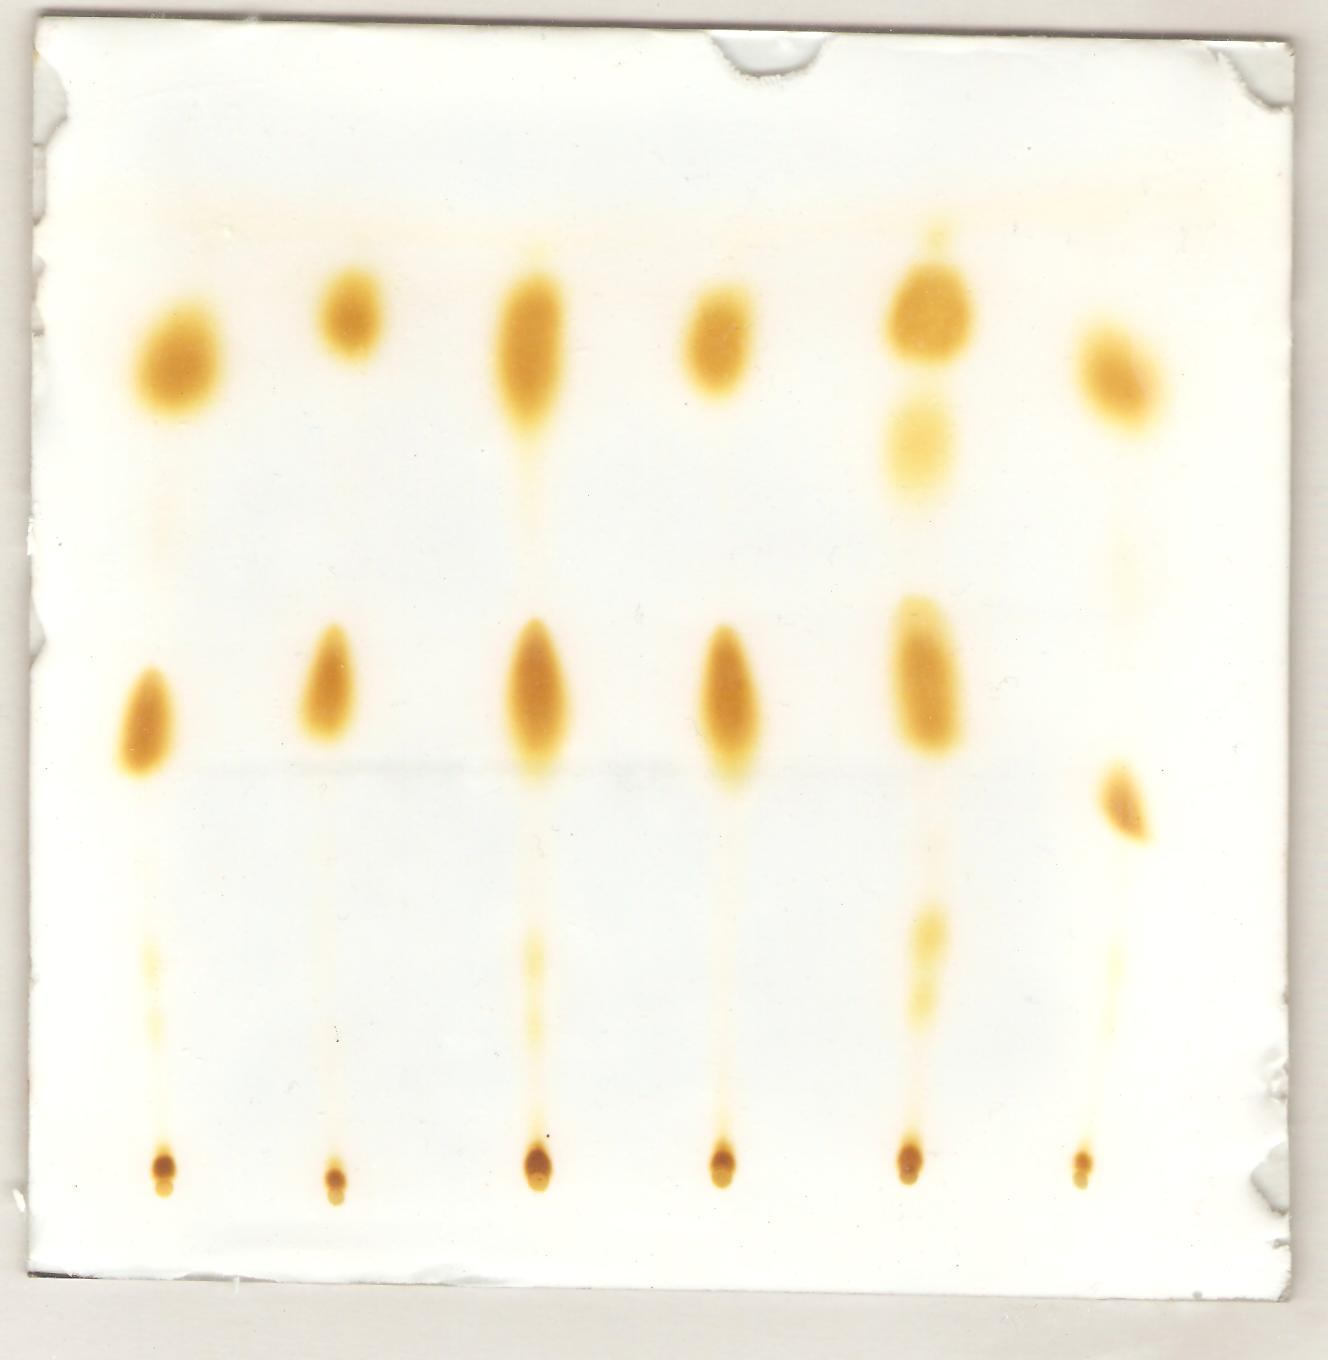
\includegraphics[width=230px]{imagenes-jtlc/experimento/fuente}
	\centering
	\vspace{-0.4cm}
	\caption{Im\'agen fuente.}
	\label{fig:image-font}
	\vspace{-0.15cm}
\end{figure}

\subsubsection{B\'usqueda de puntos de corte}
Como proceso previo se aplican los efectos de im\'agen en el siguiente orden: blur gaussiano, escala de grises, inversi\'on de colores y treshold. Se realiza un calculo de la media horizontal y vertical. A partir de cada media se busca una codificaci\'on de color que permite determinar el inicio de im\'agen de la muestra. Por ejemplo, suponga que se tiene escala de colores del 0 al 10 dentro de la media vertical, sabiendo que el inicio de la lista ser\'a el margen superior de la im\'agen. bajo el criterio que a partir de una codifcaci\'on de 5 o m\'as se puede determinar que la im\'agen real de la muestra ha iniciado. Entonces teniendo la siguiente media: 000001112222222233344555... es posible determinar que aproximadamente despu\'es de los primeros 20 puntos de la im\'agen, inicia la muestra real. Por lo tanto los primeros 20 puntos estar\'ian sobrando y se dir\'ia que a partir del punto 20 se estima un punto de corte. De forma an\'aloga se tratan el resto de los puntos de corte, el vertical inferior y los horizontales.

\begin{figure}[H]
	\vspace{-0.2cm}
	\centering
	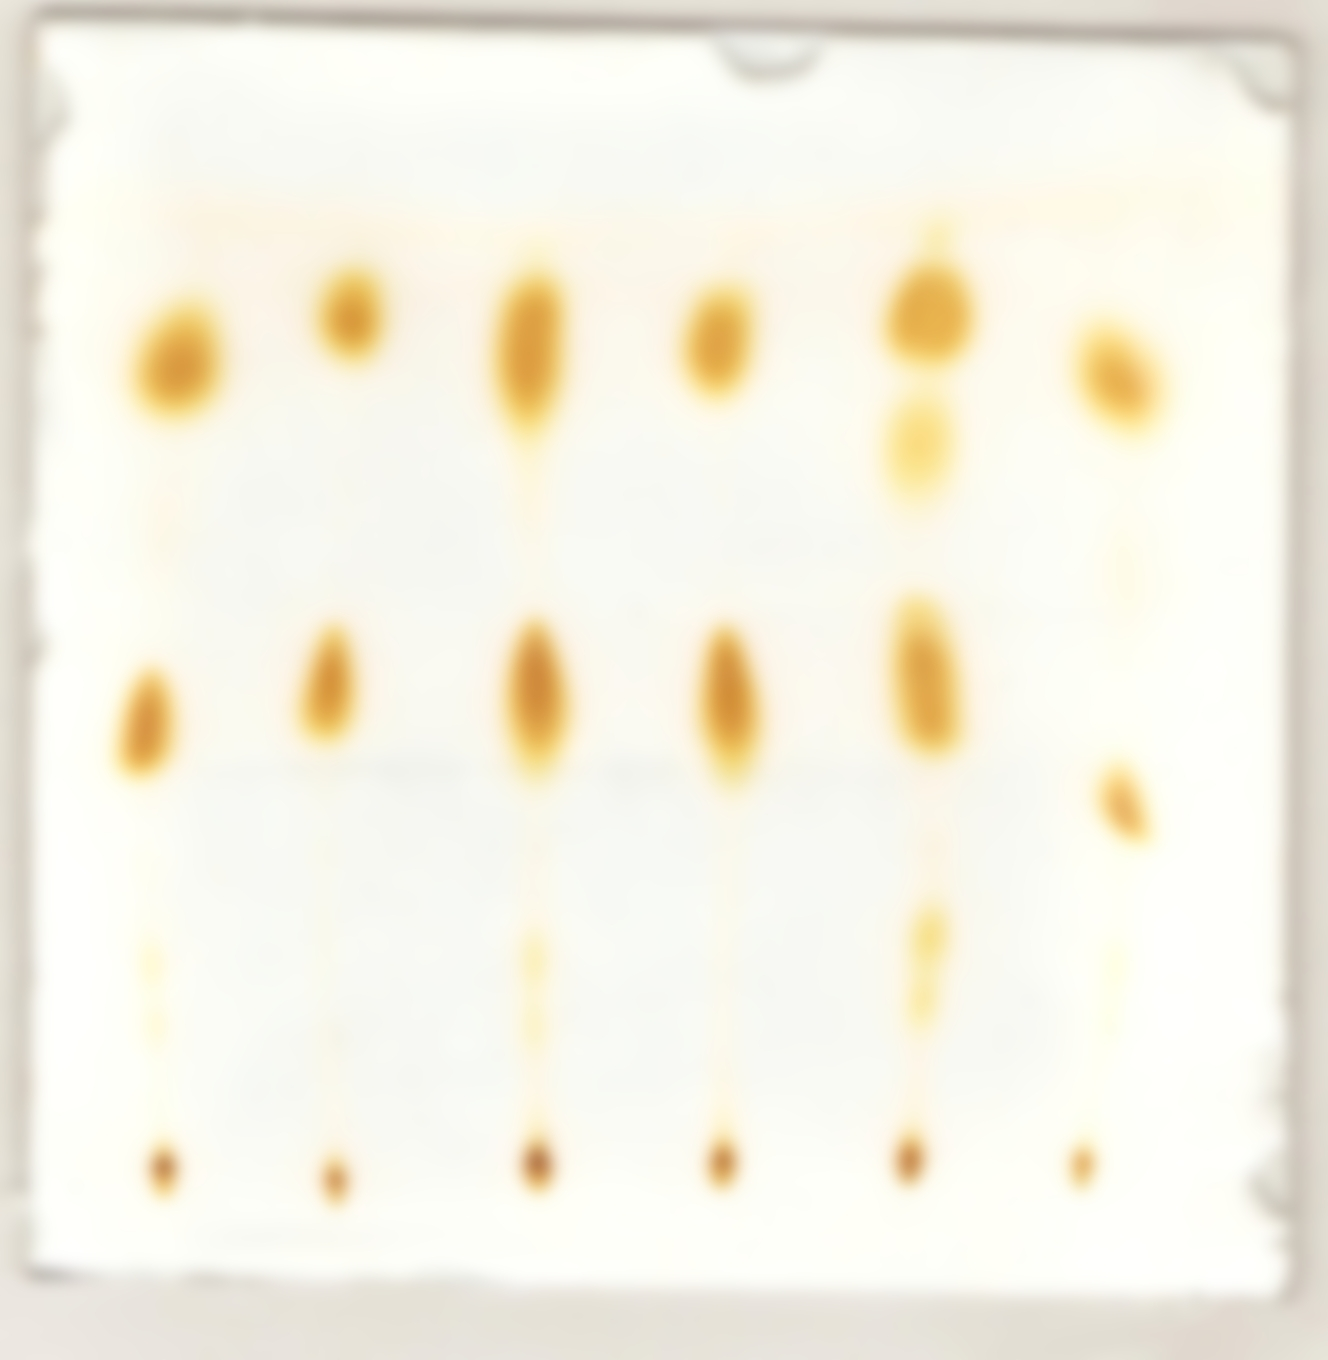
\includegraphics[width=230px]{imagenes-jtlc/experimento/search-cut-points/1-blur}
	\centering
	\vspace{-0.4cm}
	\caption{Im\'agen fuente con efecto blur aplicado.}
	\label{fig:font-blur}
	\vspace{-0.15cm}
\end{figure}
\begin{figure}[H]
	  \vspace{-0.2cm}
	  \centering
	  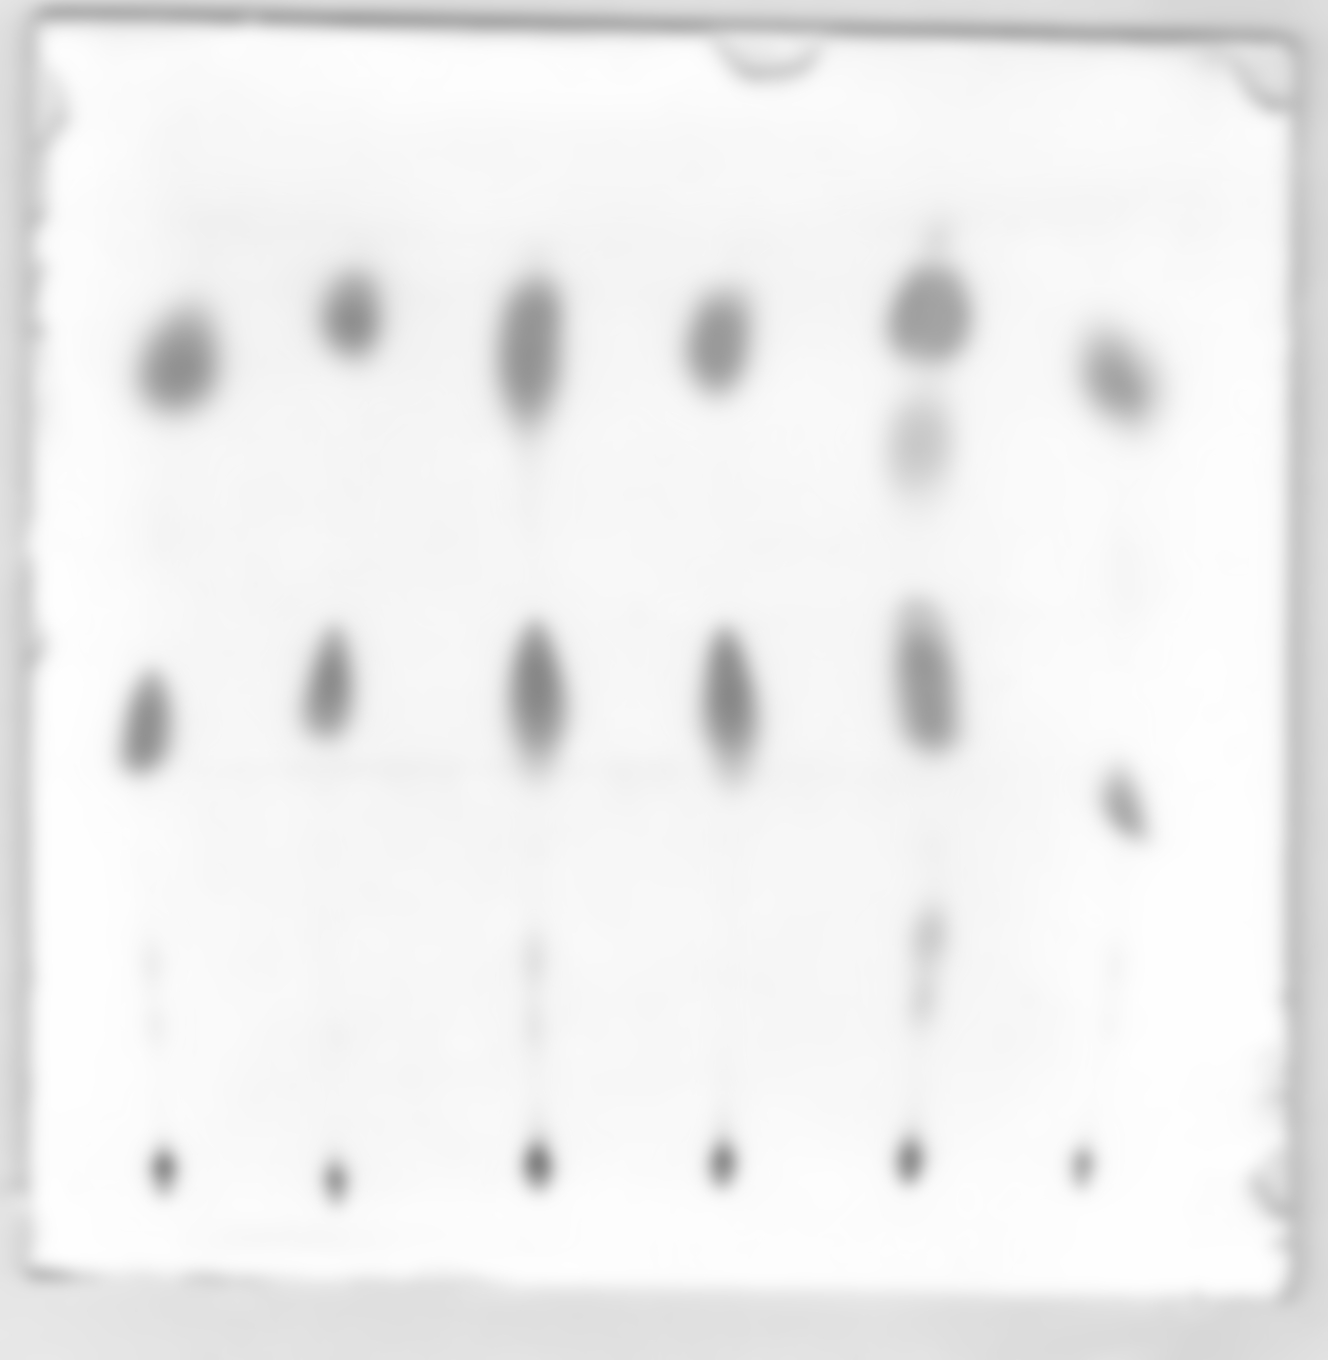
\includegraphics[width=230px]{imagenes-jtlc/experimento/search-cut-points/2-gray}
	  \centering
	  \vspace{-0.4cm}
	  \caption{Im\'agen blur con efecto escala de grises aplicado.}
	  \label{fig:font-gray}
	  \vspace{-0.15cm}
\end{figure}
\begin{figure}[H]
	  \vspace{-0.2cm}
	  \centering
	  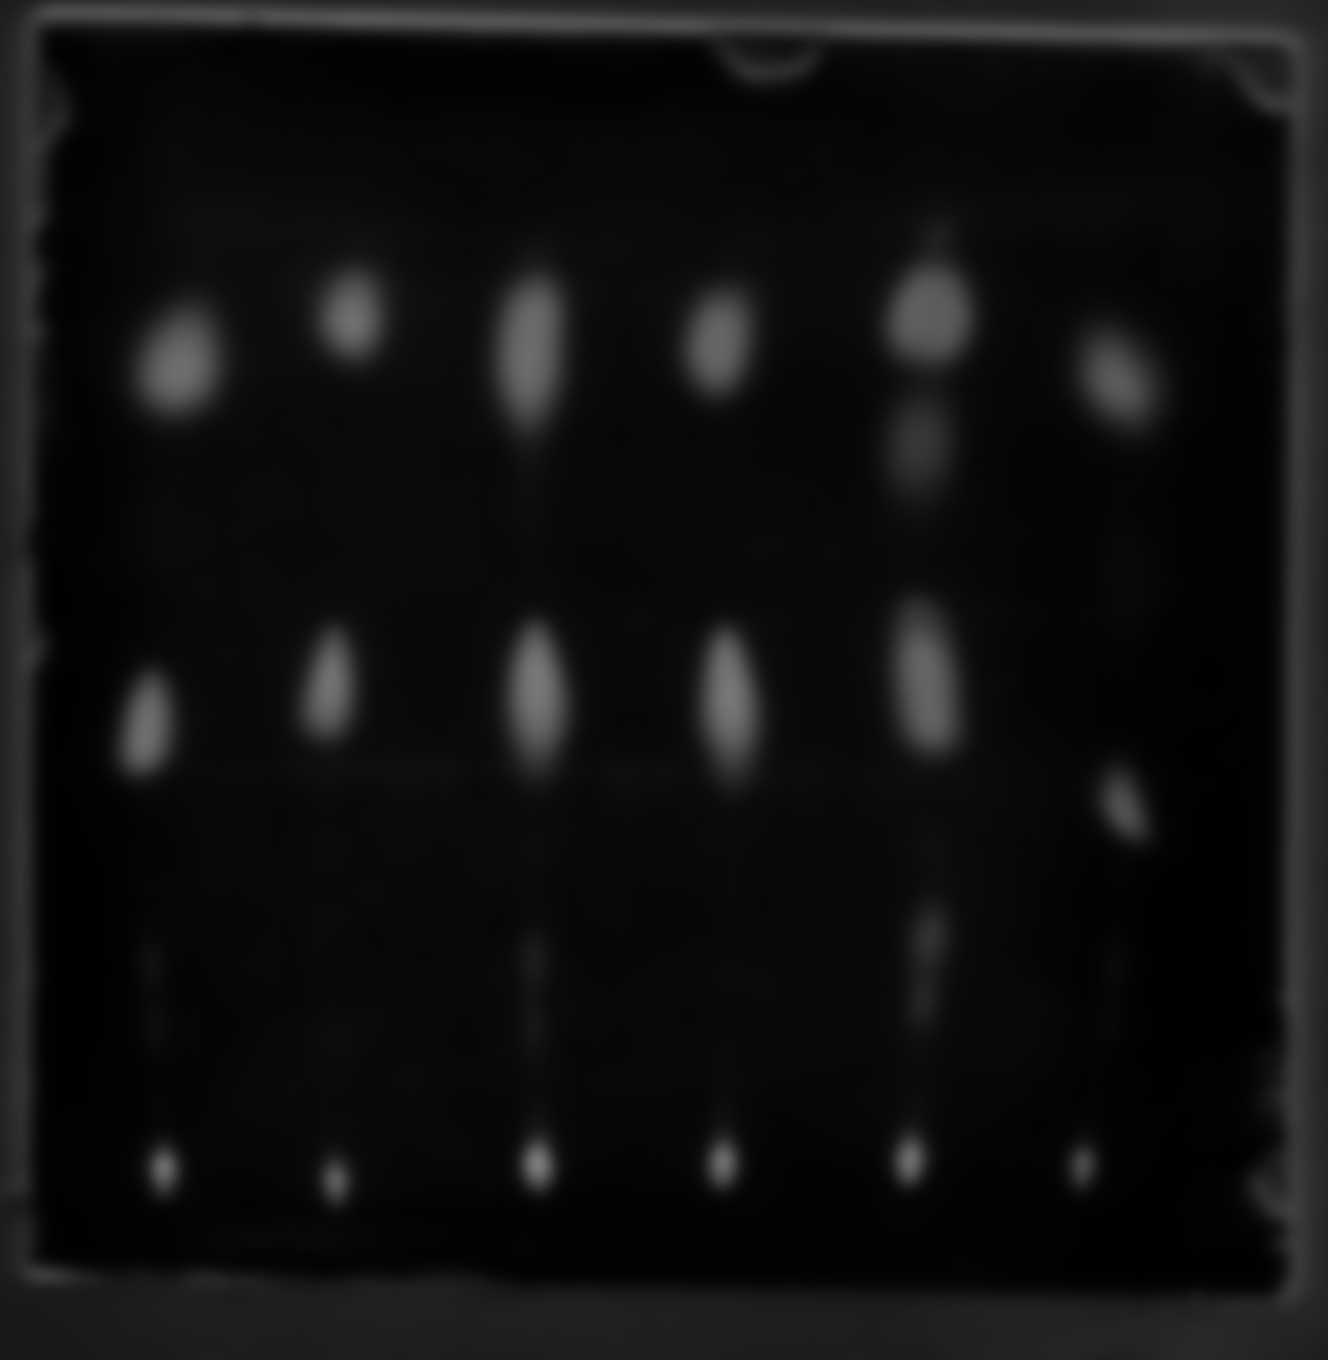
\includegraphics[width=230px]{imagenes-jtlc/experimento/search-cut-points/3-invert}
	  \centering
	  \vspace{-0.4cm}
	  \caption{Im\'agen blur-gray con efecto colores invertidos aplicado.}
	  \label{fig:font-invert}
	  \vspace{-0.15cm}
\end{figure}
\begin{figure}[H]
	  \vspace{-0.2cm}
	  \centering
	  \fbox{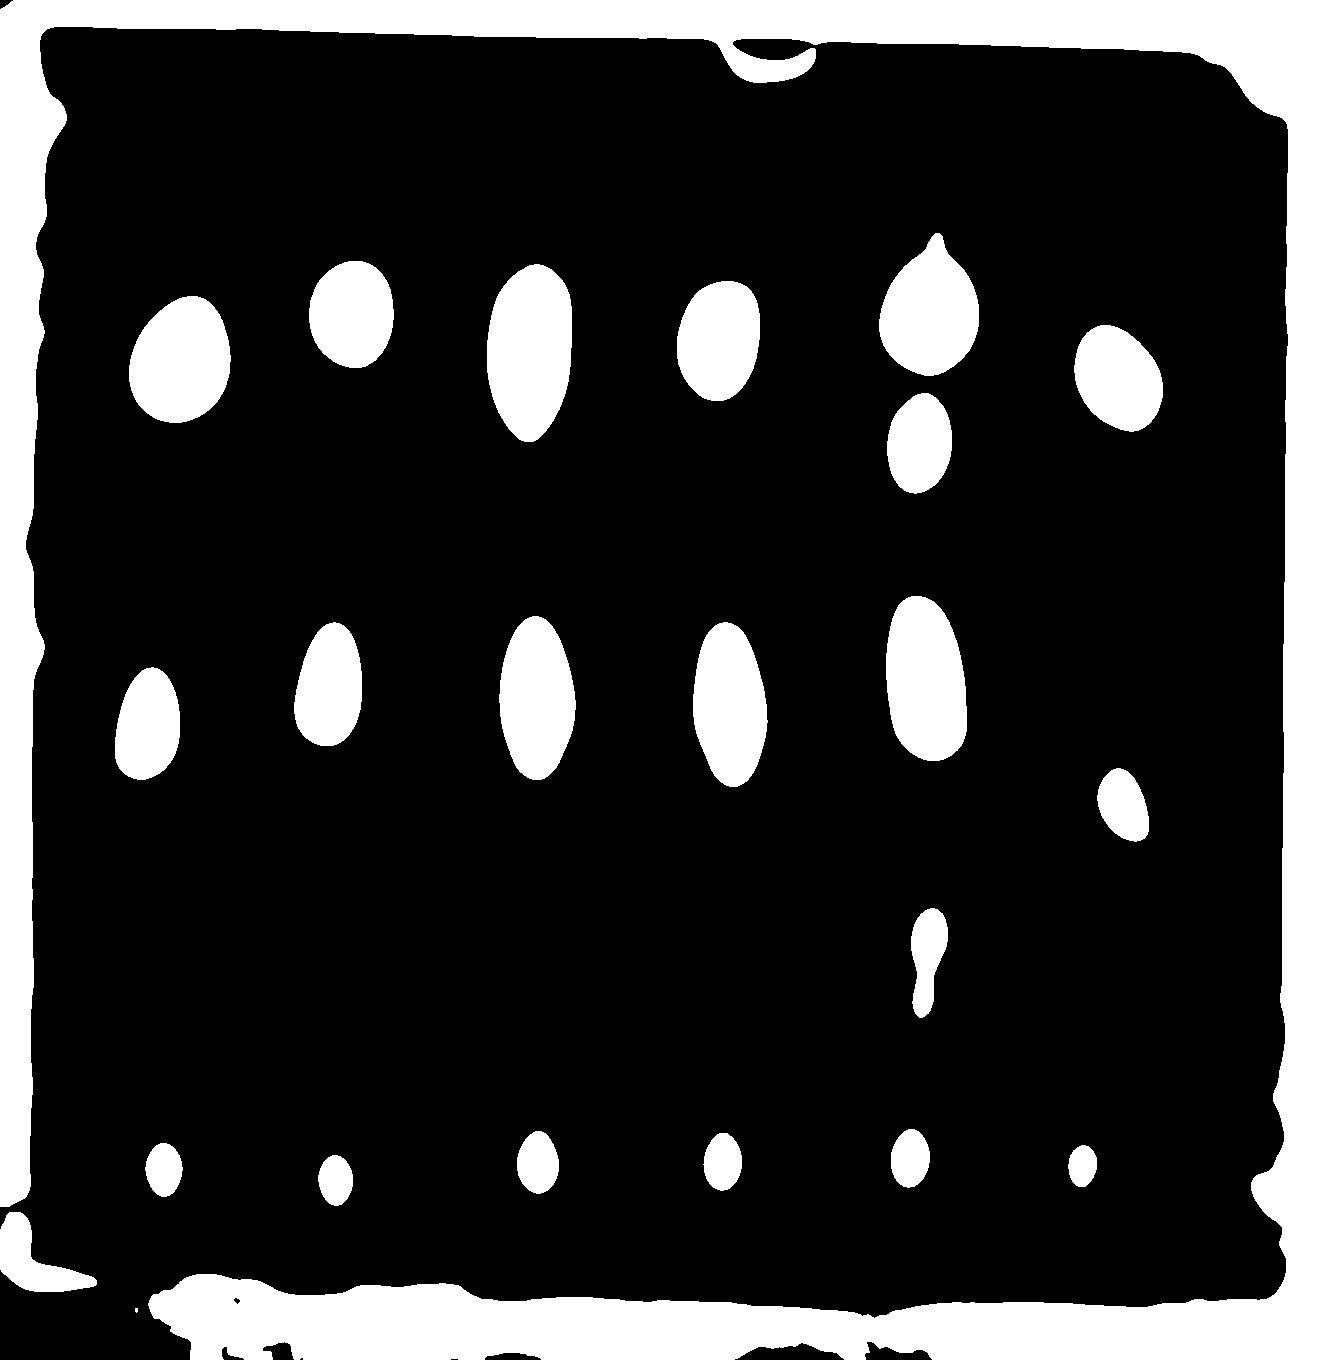
\includegraphics[width=230px]{imagenes-jtlc/experimento/search-cut-points/4-threshold}}
	  \centering
	  \vspace{-0.4cm}
	  \caption{Im\'agen blur-gray-invert con efecto threshold aplicado.}
	  \label{fig:font-thresh}
	  \vspace{-0.15cm}
\end{figure}
\begin{figure}[H]
	  \vspace{-0.2cm}
	  \centering
	  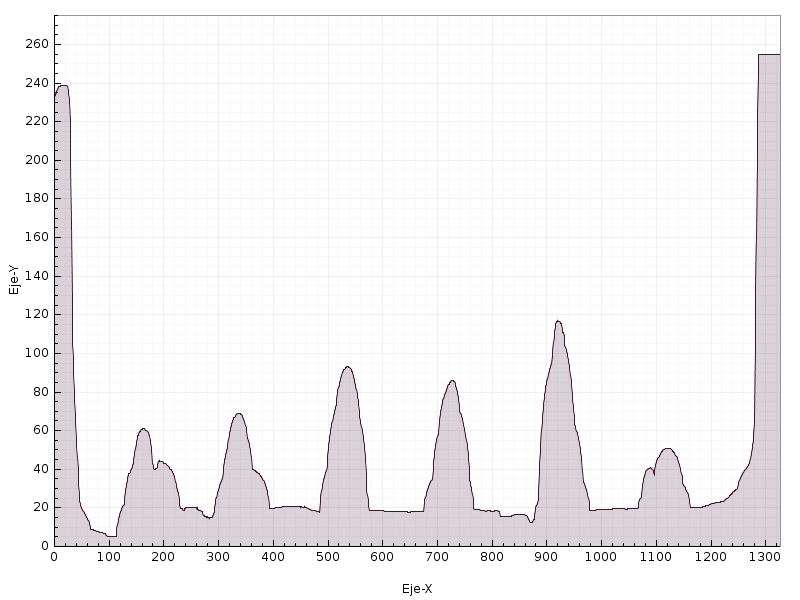
\includegraphics[width=230px]{imagenes-jtlc/experimento/search-cut-points/plot-x}
	  \centering
	  \vspace{-0.4cm}
	  \caption{Plot de media sobre im\'agen con efectos en eje X.}
	  \label{fig:font-sc-plot-x}
	  \vspace{-0.15cm}
\end{figure}
\begin{figure}[H]
	  \vspace{-0.2cm}
	  \centering
	  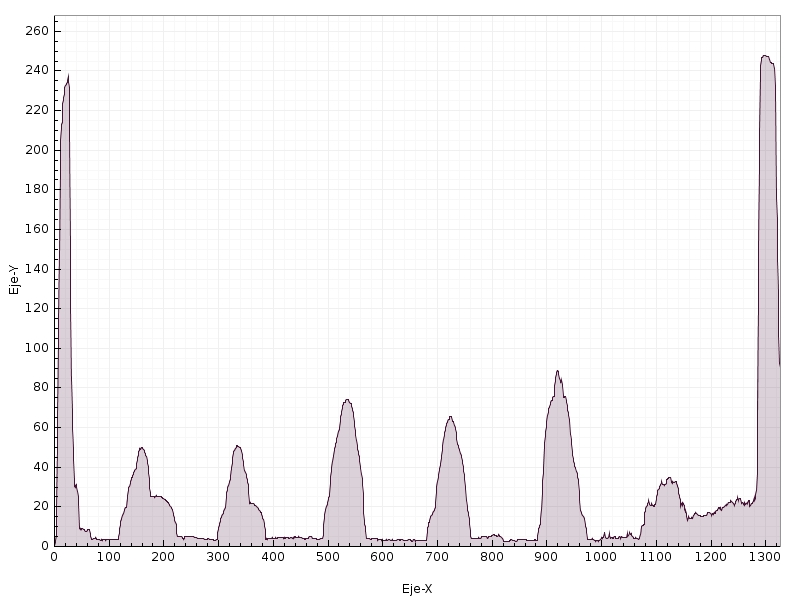
\includegraphics[width=230px]{imagenes-jtlc/experimento/search-cut-points/plot-x-no-blur}
	  \centering
	  \vspace{-0.4cm}
	  \caption{Plot de media sobre im\'agen con efectos (sin blur) en eje X.}
	  \label{fig:font-sc-plot-x-s-blur}
	  \vspace{-0.15cm}
\end{figure}
\begin{figure}[H]
	  \vspace{-0.2cm}
	  \centering
	  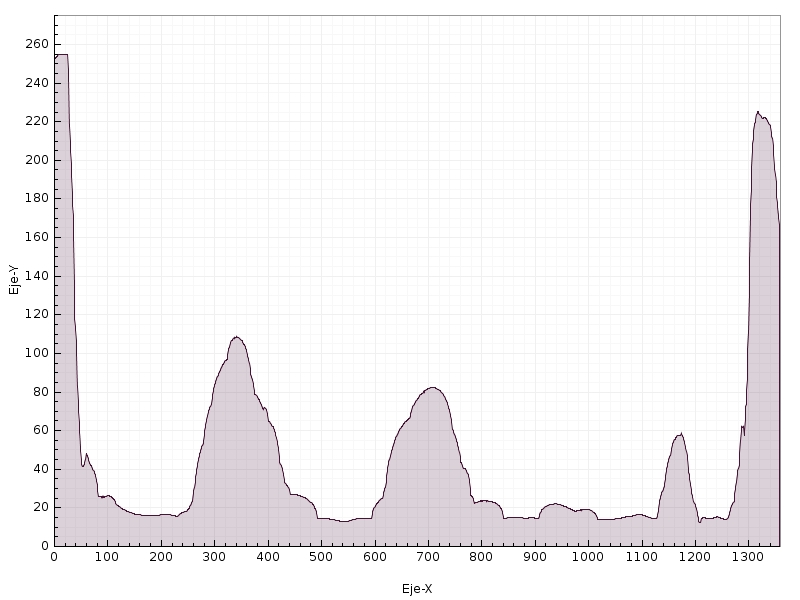
\includegraphics[width=230px]{imagenes-jtlc/experimento/search-cut-points/plot-y}
	  \centering
	  \vspace{-0.4cm}
	  \caption{Plot de media sobre im\'agen con efectos en eje Y.}
	  \label{fig:font-sc-plot-y}
	  \vspace{-0.15cm}
\end{figure}
\begin{figure}[H]
	  \vspace{-0.2cm}
	  \centering
	  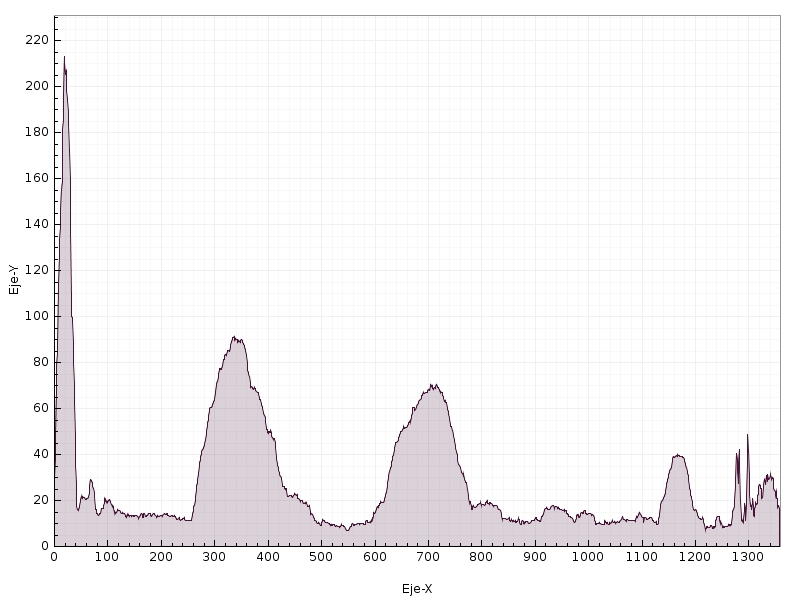
\includegraphics[width=230px]{imagenes-jtlc/experimento/search-cut-points/plot-y-no-blur}
	  \centering
	  \vspace{-0.4cm}
	  \caption{Plot de media sobre im\'agen con efectos (sin blur) en eje Y.}
	  \label{fig:font-sc-plot-y-s-blur}
	  \vspace{-0.15cm}
\end{figure}
Puntos de corte encontrados:\\
top: (73, 135) \\
bottom: (1216, 1261) \\

\subsubsection{B\'usqueda de muestras}
Como proceso previo se aplican los efectos de im\'agen en el siguiente orden: blur gaussiano, escala de grises, inversi\'on de colores y treshold. Se codifica la im\'agen desde una perspectiva vertical en ceros y unos para determinar las zonas con color, esto permite delimitar las zonas verticales donde existen muestras. A continuaci\'on se mostrar\'a el ejemplo de una codificaci\'on y una interpretaci\'on de la misma.
\newpage
\begin{center}
- - - - - - - - - -\\
0 0 0 1 0 0 0 0 1 0\\
0 0 1 1 0 0 0 0 1 0\\
0 0 0 0 0 0 1 0 0 0\\
- - - - - - - - - -\\
1 0 1 1 0 0 1 0 1 0\\
\end{center}

Debajo de la l\'inea de puntos se aprecia el resultado de la codificaci\'on. Entonces podr\'ian determinarse cuatro \'areas de muestra seg\'un el ejemplo, generadas por las subsecuencias de unos en el resultado. De este modo se toman los \'indices correspondientes con los que se determinan las \'areas sobre la im\'agen real. 


\subsubsection{B\'usqueda de picos}
Como proceso previo se aplican los efectos de im\'agen en el siguiente orden: blur gaussiano, escala de grises e inversi\'on de colores. Luego de aplicar los filtros, se realiza el siguiente proceso en cada muestra: se realiza el c\'omputo de la media desde una perspectiva horizontal y con esta lista de valores que representa  a la parte m\'as larga de la im\'agen que se considera la muestra se buscar\'an los picos. Dichos picos tendr\'an un alto m\'inimo para considerarse como tal. En un principio se realiza la b\'usqueda de un pico considerando el m\'aximo de la lista que no se ha analizado. En base a este m\'aximo se hace una b\'usqueda por izquierda y por derecha de un punto de inflexi\'on, es decir, si se busca por izquierda del m\'aximo, los valores decrecen con cierto \'angulo de decrecimiento pero llegar\'a el momento en que este \'angulo se invierta o bien cobre estabilidad en sus valores (esto se analiza en base al gradiente obtenido entre los puntos), se puede decir que all\'i hay un punto de inflexi\'on. Luego se realiza el mismo proceso hacia el lado derecho del m\'aximo, se guardan los valores de puntos de inflexi\'on y el \'area que se encuentra entre dichos puntos (que contienen al m\'aximo del pico) se considera como \'area en la que se realizar\'an los c\'alculos futuros del an\'alisis, \'areas de integraci\'on. Dentro del an\'alisis de \'areas se realizan correcciones para evitar \'areas superpuestas considerando un punto medio que separe a ambas.
Como parte de la b\'usqueda de picos se realiza adem\'as un c\'alculo extra en el que se determina la l\'inea base de cada \'area, la cual est\'a definida por la recta que se forma entre cada punto de inflexi\'on pero sin tener en cuenta aquellos puntos que corten la l\'inea de la curva.

\subsubsection{Integraci\'on del \'area}
Una vez obtenidos los picos y las l\'ineas base correspondiente se procede a realizar la integraci\'on del \'area sumando el \'area que hay bajo la funci\'on de la curva pero teniendo el cuenta adem\'as el \'area que est\'a por encima de la l\'inea base.

\subsubsection{Ejemplo del procesado de im\'agenes y resultados parciales}
QUITAR y DISTRIBUIR EN LAS SECCIONES SUPERIORES\\
A continuaci\'on se presentar\'a un ejemplo en el que se podr\'a ver la im\'agen fuente del experimento y el proceso que recibe antes de llegar al resultado final.
\begin{itemize}
	\renewcommand{\labelitemi}{$\bullet$}
	\renewcommand{\labelitemii}{$\circ$}
	

	\item \textit{B\'usqueda de puntos de corte}
	
	\newpage
	\item \textit{B\'usqueda de muestras}
	\begin{figure}[H]
	  \vspace{-0.2cm}
	  \centering
	  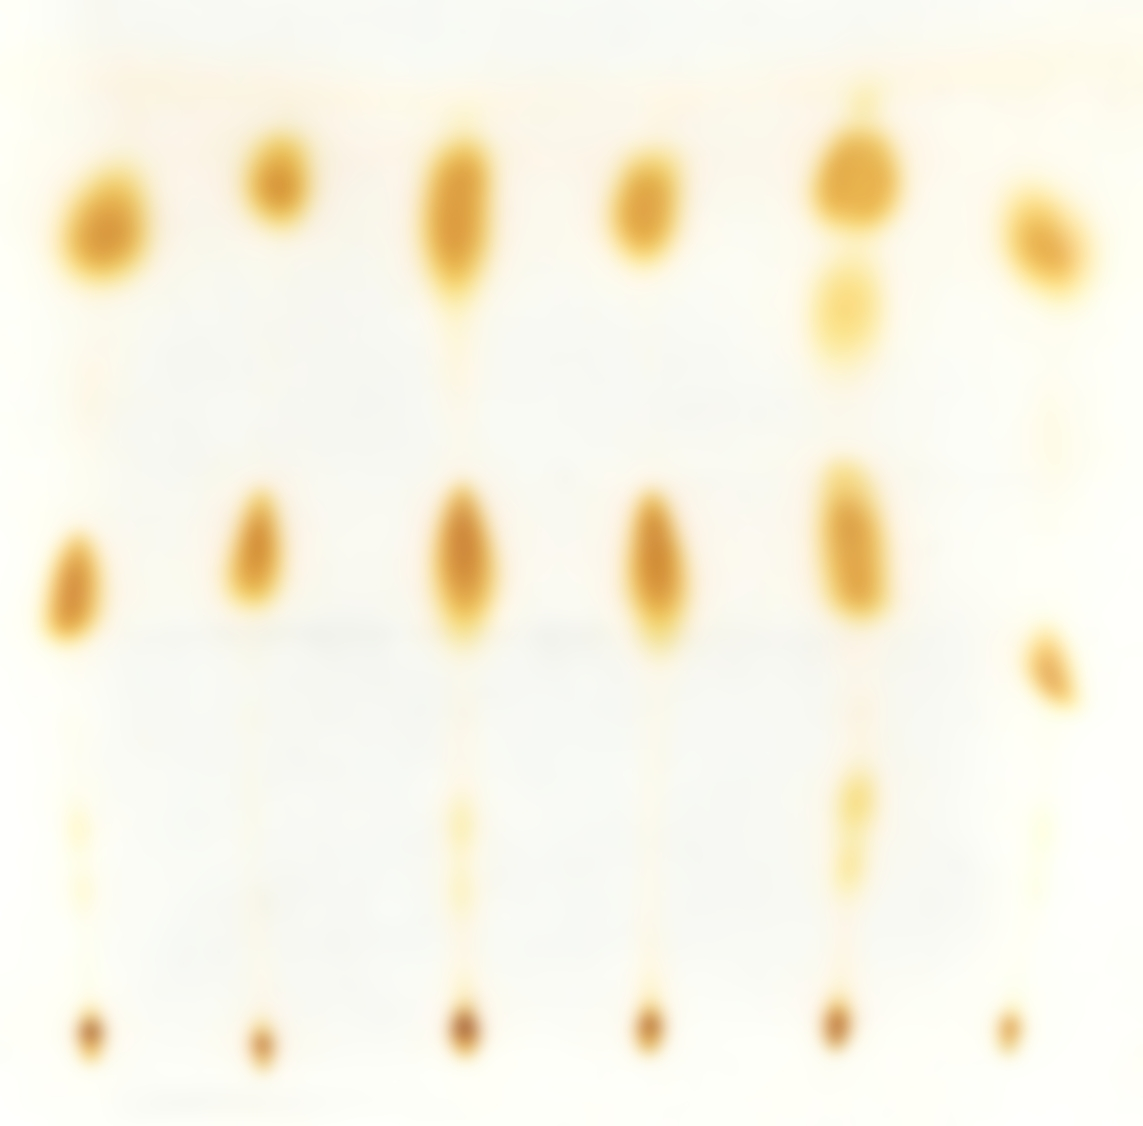
\includegraphics[width=230px]{imagenes-jtlc/experimento/search-samples/1-blur}
	  \centering
	  \vspace{-0.4cm}
	  \caption{Im\'agen fuente con efecto blur aplicado.}
	  \label{fig:font-c-blur}
	  \vspace{-0.15cm}
	\end{figure}
	\begin{figure}[H]
	  \vspace{-0.2cm}
	  \centering
	  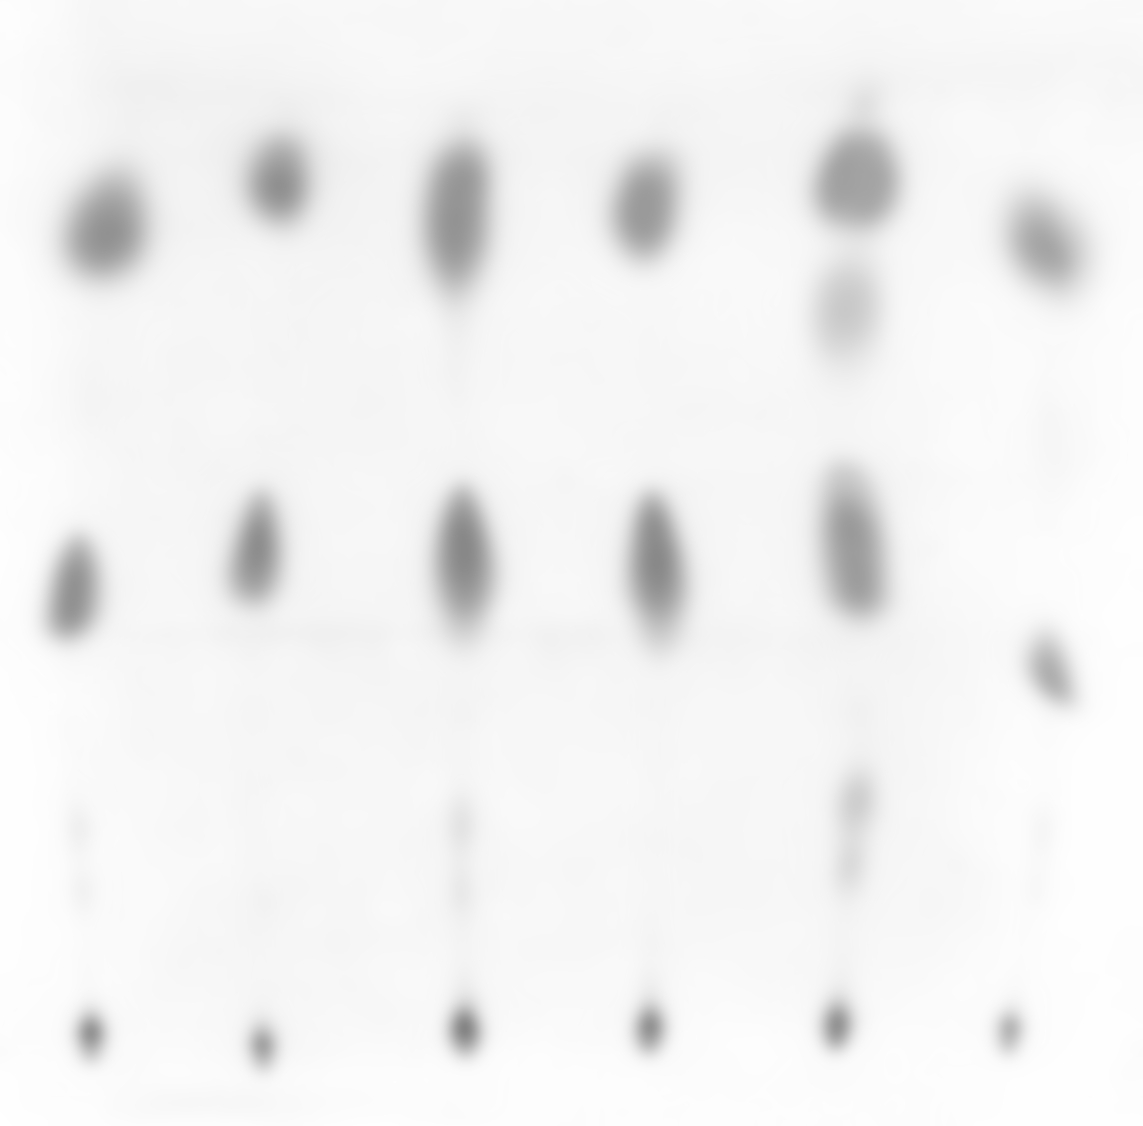
\includegraphics[width=230px]{imagenes-jtlc/experimento/search-samples/2-gray}
	  \centering
	  \vspace{-0.4cm}
	  \caption{Im\'agen blur con efecto escala de grises aplicado.}
	  \label{fig:font-c-gray}
	  \vspace{-0.15cm}
	\end{figure}
	\begin{figure}[H]
	  \vspace{-0.2cm}
	  \centering
	  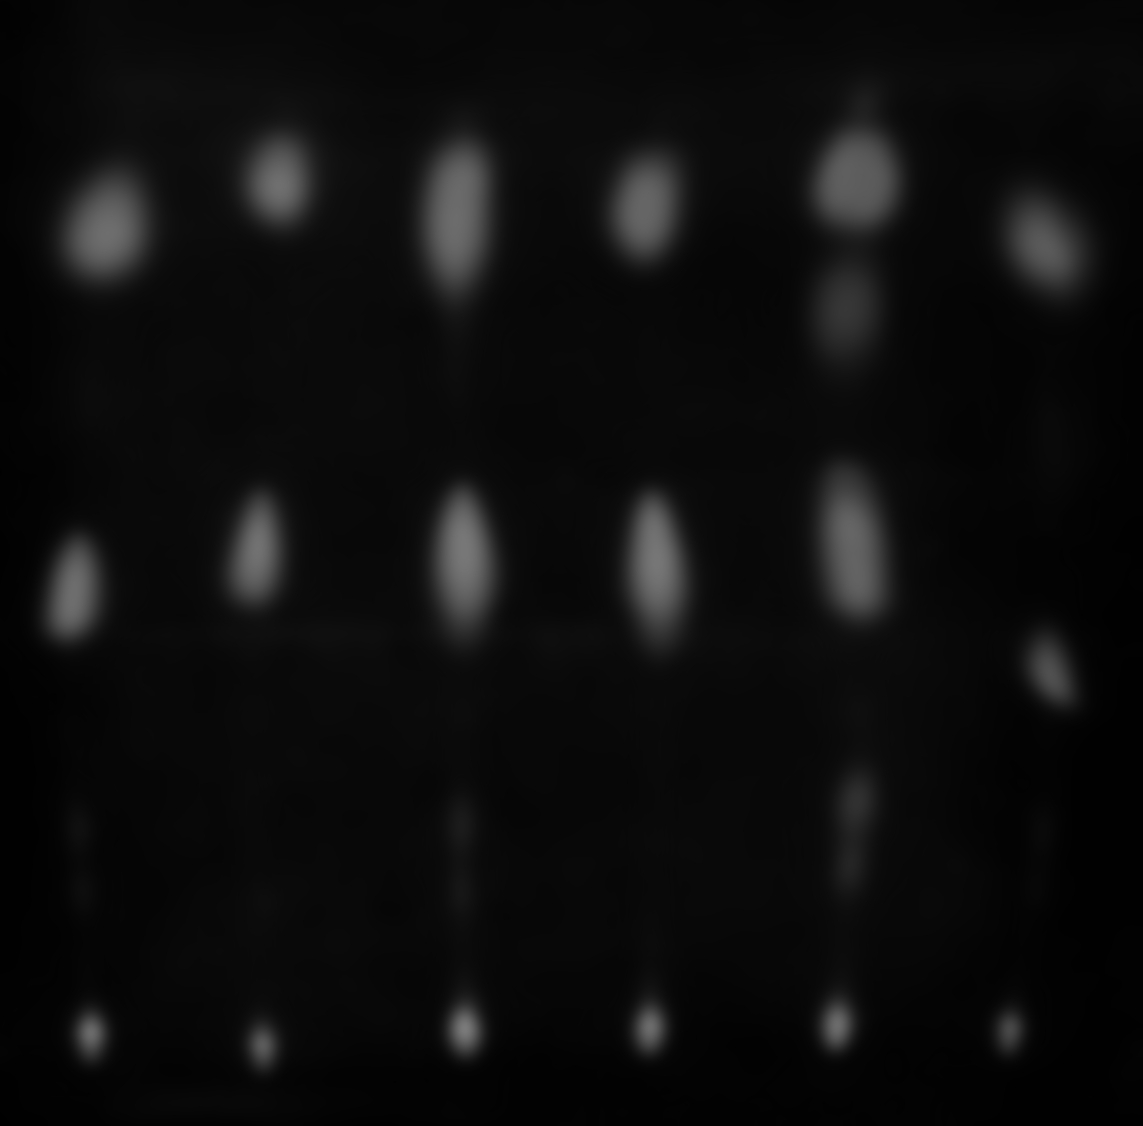
\includegraphics[width=230px]{imagenes-jtlc/experimento/search-samples/3-invert}
	  \centering
	  \vspace{-0.4cm}
	  \caption{Im\'agen blur-gray con efecto colores invertidos aplicado.}
	  \label{fig:font-c-invert}
	  \vspace{-0.15cm}
	\end{figure}
	\begin{figure}[H]
	  \vspace{-0.2cm}
	  \centering
	  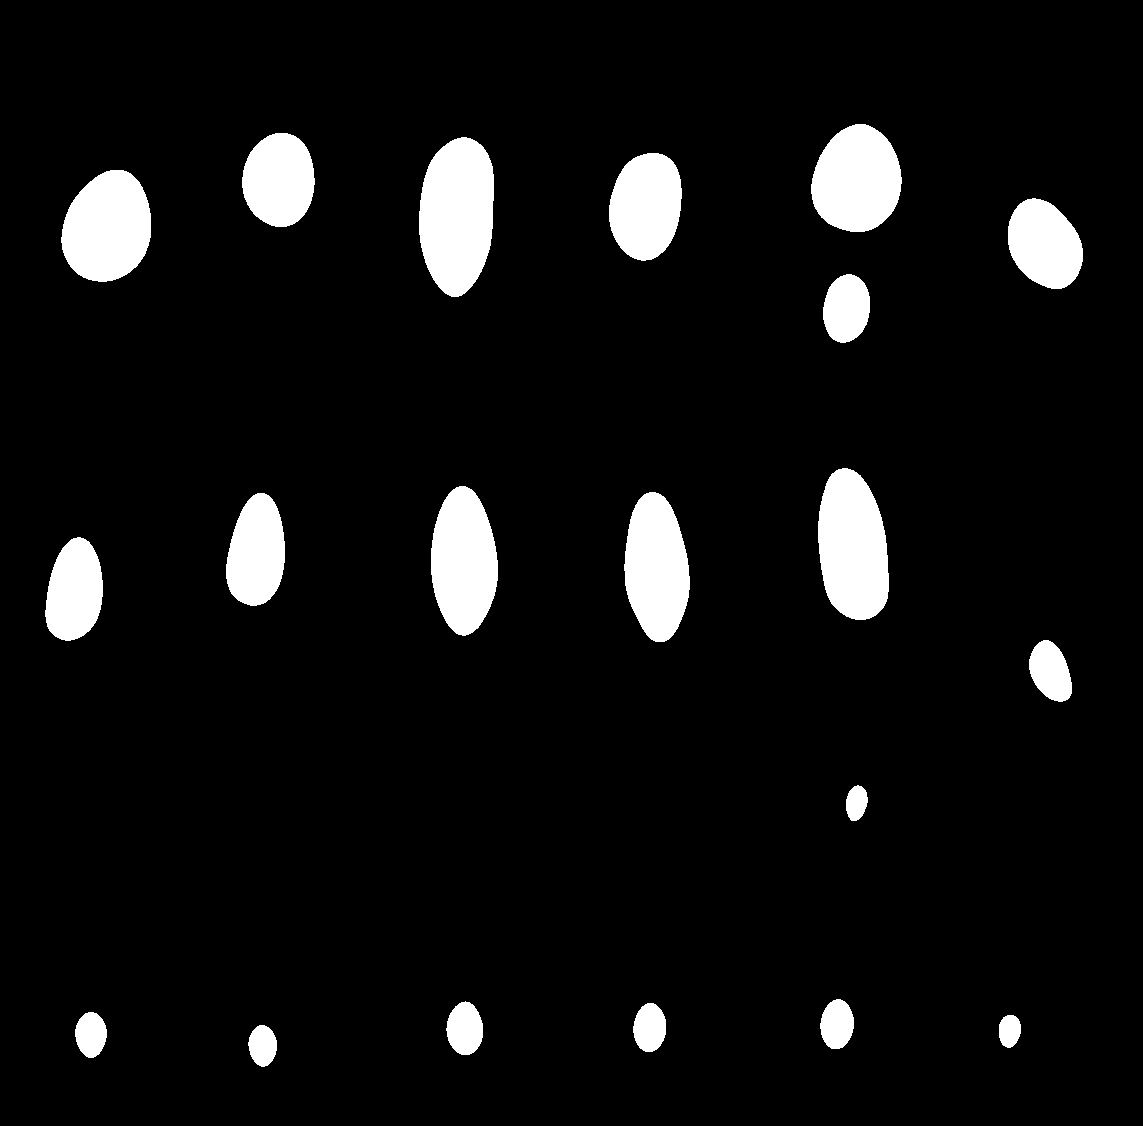
\includegraphics[width=230px]{imagenes-jtlc/experimento/search-samples/4-threshold}
	  \centering
	  \vspace{-0.4cm}
	  \caption{Im\'agen blur-gray-invert con efecto threshold aplicado.}
	  \label{fig:font-c-thresh}
	  \vspace{-0.15cm}
	\end{figure}
	\begin{figure}[H]
	  \vspace{-0.2cm}
	  \centering
	  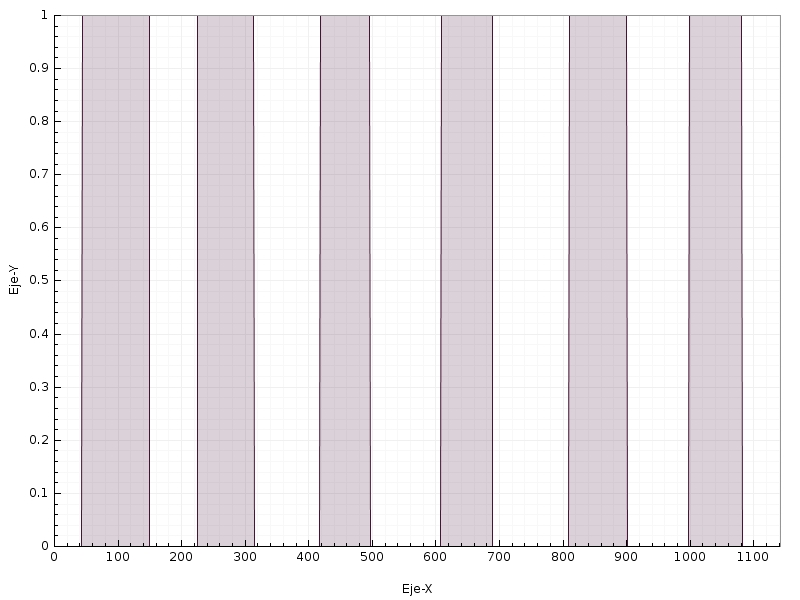
\includegraphics[width=230px]{imagenes-jtlc/experimento/search-samples/plot-y}
	  \centering
	  \vspace{-0.4cm}
	  \caption{Plot de media sobre im\'agen con efectos en eje Y.}
	  \label{fig:font-c-plot-y}
	  \vspace{-0.15cm}
	\end{figure}
	Muestras encontradas (puntos sobre eje-x):\\
	(45, 150)\\
	(226, 314)\\
	(419, 497)\\
	(609, 689)\\
	(811, 901)\\
	(999, 1082)\\
	
	\newpage
	\item \textit{B\'usqueda de picos (muestra 1)}
	\begin{figure}[H]
	\centering
	\fbox{
\includegraphics[width=40px]{imagenes-jtlc/experimento/search-peaks/1/1-blur}}   
	\hspace{30px}
	\fbox{
\includegraphics[width=40px]{imagenes-jtlc/experimento/search-peaks/1/2-gray}}
	\hspace{30px}
	\fbox{
\includegraphics[width=40px]{imagenes-jtlc/experimento/search-peaks/1/3-invert}}
	\caption{Aplicaci\'on de filtros sobre im\'agen de la muestra}
	\centering
	\end{figure}
	\begin{figure}[H]
	  \vspace{-0.2cm}
	  \centering
	  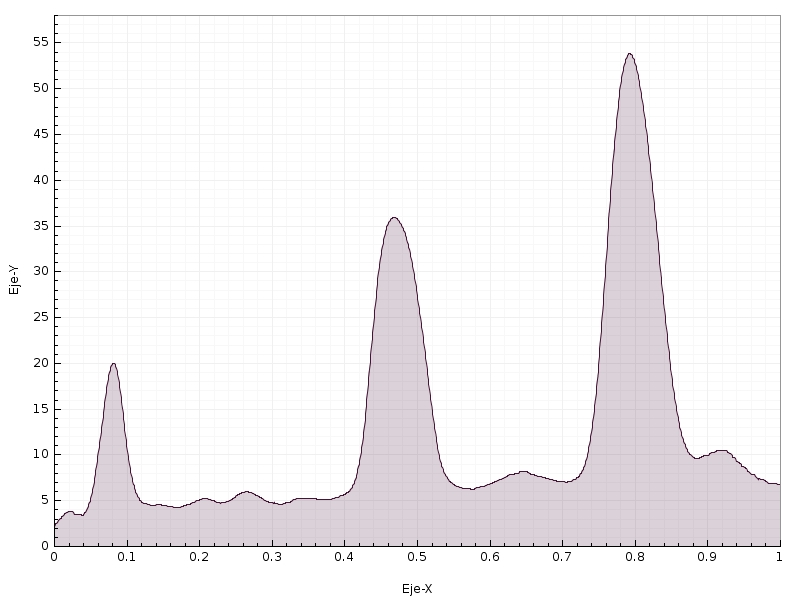
\includegraphics[width=230px]{imagenes-jtlc/experimento/search-peaks/1/plot-x}
	  \centering
	  \vspace{-0.4cm}
	  \caption{Plot de media sobre im\'agen con efectos en eje X.}
	  \label{fig:sp-1-plot-x}
	  \vspace{-0.15cm}
	\end{figure}
	\begin{figure}[H]
	  \vspace{-0.2cm}
	  \centering
	  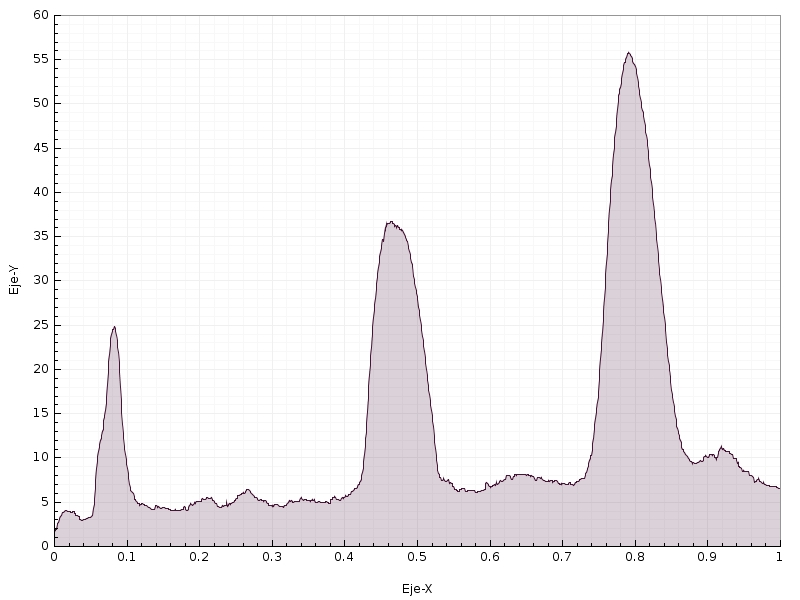
\includegraphics[width=230px]{imagenes-jtlc/experimento/search-peaks/1/plot-x-no-blur}
	  \centering
	  \vspace{-0.4cm}
	  \caption{Plot de media sobre im\'agen con efectos (sin blur) en eje X.}
	  \label{fig:sp-1-plot-x-no-blur}
	  \vspace{-0.15cm}
	\end{figure}
	Picos encontrados:\\
	(0.42933333, 0.53333336)\\
	(0.73422223, 0.8702222)\\ \\
	Picos encontrados (sin blur):\\
	(0.43733335, 0.47111112)\\
	(0.47111112, 0.52177775)\\
	(0.72, 0.86755556)\\
	
	\newpage
	\item \textit{B\'usqueda de picos (muestra 2)}
	\begin{figure}[H]
	\centering
	\fbox{
\includegraphics[width=40px]{imagenes-jtlc/experimento/search-peaks/2/1-blur}}   
	\hspace{30px}
	\fbox{
\includegraphics[width=40px]{imagenes-jtlc/experimento/search-peaks/2/2-gray}}
	\hspace{30px}
	\fbox{
\includegraphics[width=40px]{imagenes-jtlc/experimento/search-peaks/2/3-invert}}
	\caption{Aplicaci\'on de filtros sobre im\'agen de la muestra}
	\centering
	\end{figure}
	\begin{figure}[H]
	  \vspace{-0.2cm}
	  \centering
	  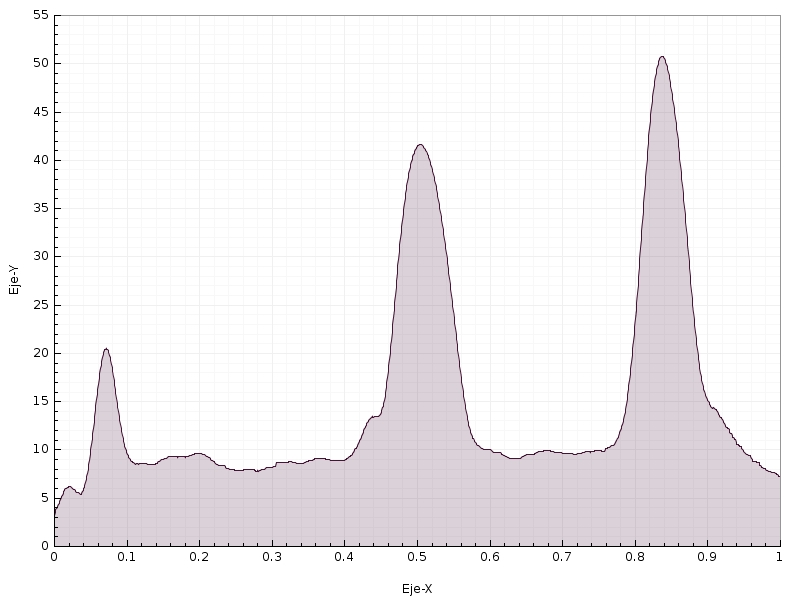
\includegraphics[width=230px]{imagenes-jtlc/experimento/search-peaks/2/plot-x}
	  \centering
	  \vspace{-0.4cm}
	  \caption{Plot de media sobre im\'agen con efectos en eje X.}
	  \label{fig:sp-2-plot-x}
	  \vspace{-0.15cm}
	\end{figure}
	\begin{figure}[H]
	  \vspace{-0.2cm}
	  \centering
	  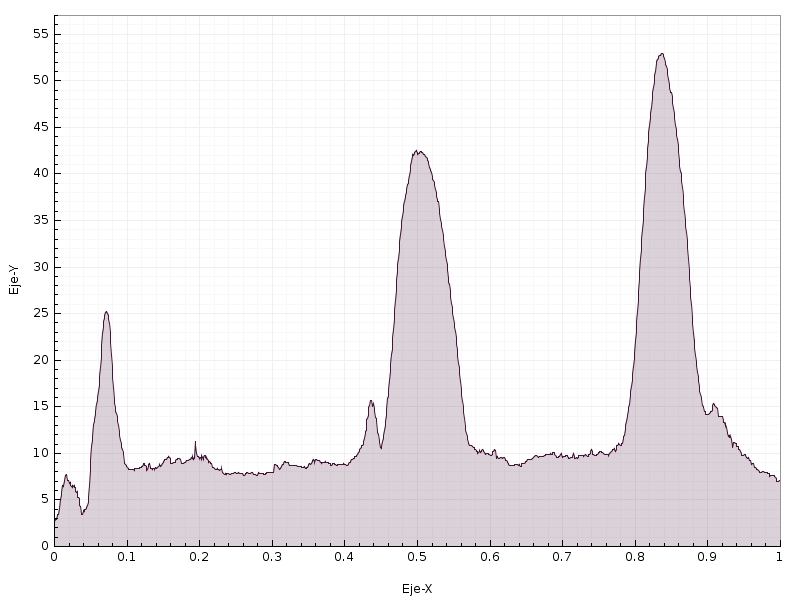
\includegraphics[width=230px]{imagenes-jtlc/experimento/search-peaks/2/plot-x-no-blur}
	  \centering
	  \vspace{-0.4cm}
	  \caption{Plot de media sobre im\'agen con efectos (sin blur) en eje X.}
	  \label{fig:sp-2-plot-x-no-blur}
	  \vspace{-0.15cm}
	\end{figure}
	Picos encontrados: \\
	(0.4231111, 0.5742222)\\
	(0.7911111, 0.97422224)\\ \\
	Picos encontrados (sin blur):\\
	(0.46222222, 0.5004445)\\
	(0.5004445, 0.55644447)\\
	(0.77511114, 0.8977778)\\
	
	\item \textit{B\'usqueda de picos (muestra 3)}
	\begin{figure}[H]
	\centering
	\fbox{
\includegraphics[width=40px]{imagenes-jtlc/experimento/search-peaks/3/1-blur}}   
	\hspace{30px}
	\fbox{
\includegraphics[width=40px]{imagenes-jtlc/experimento/search-peaks/3/2-gray}}
	\hspace{30px}
	\fbox{
\includegraphics[width=40px]{imagenes-jtlc/experimento/search-peaks/3/3-invert}}
	\caption{Aplicaci\'on de filtros sobre im\'agen de la muestra}
	\centering
	\end{figure}
	\begin{figure}[H]
	  \vspace{-0.2cm}
	  \centering
	  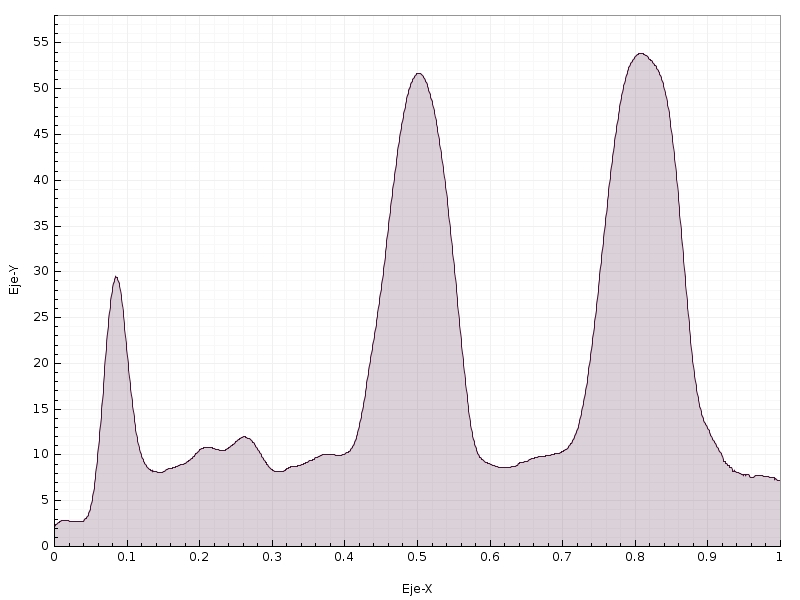
\includegraphics[width=230px]{imagenes-jtlc/experimento/search-peaks/3/plot-x}
	  \centering
	  \vspace{-0.4cm}
	  \caption{Plot de media sobre im\'agen con efectos en eje X.}
	  \label{fig:sp-3-plot-x}
	  \vspace{-0.15cm}
	\end{figure}
	\begin{figure}[H]
	  \vspace{-0.2cm}
	  \centering
	  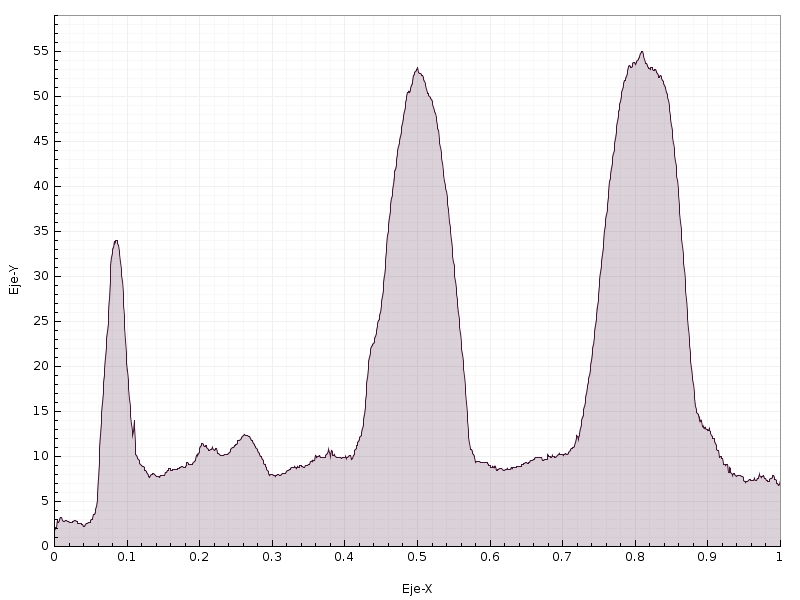
\includegraphics[width=230px]{imagenes-jtlc/experimento/search-peaks/3/plot-x-no-blur}
	  \centering
	  \vspace{-0.4cm}
	  \caption{Plot de media sobre im\'agen con efectos (sin blur) en eje X.}
	  \label{fig:sp-3-plot-x-no-blur}
	  \vspace{-0.15cm}
	\end{figure}
	Picos encontrados:\\
	(0.4328889, 0.57688886)\\
	(0.7351111, 0.9208889)\\ \\
	Picos encontrados (sin blur): \\
	(0.7457778, 0.8008889)\\
	
	\newpage
	\item \textit{B\'usqueda de picos (muestra 4)}
	\begin{figure}[H]
	\centering
	\fbox{
\includegraphics[width=40px]{imagenes-jtlc/experimento/search-peaks/4/1-blur}}   
	\hspace{30px}
	\fbox{
\includegraphics[width=40px]{imagenes-jtlc/experimento/search-peaks/4/2-gray}}
	\hspace{30px}
	\fbox{
\includegraphics[width=40px]{imagenes-jtlc/experimento/search-peaks/4/3-invert}}
	\caption{Aplicaci\'on de filtros sobre im\'agen de la muestra}
	\centering
	\end{figure}
	\begin{figure}[H]
	  \vspace{-0.2cm}
	  \centering
	  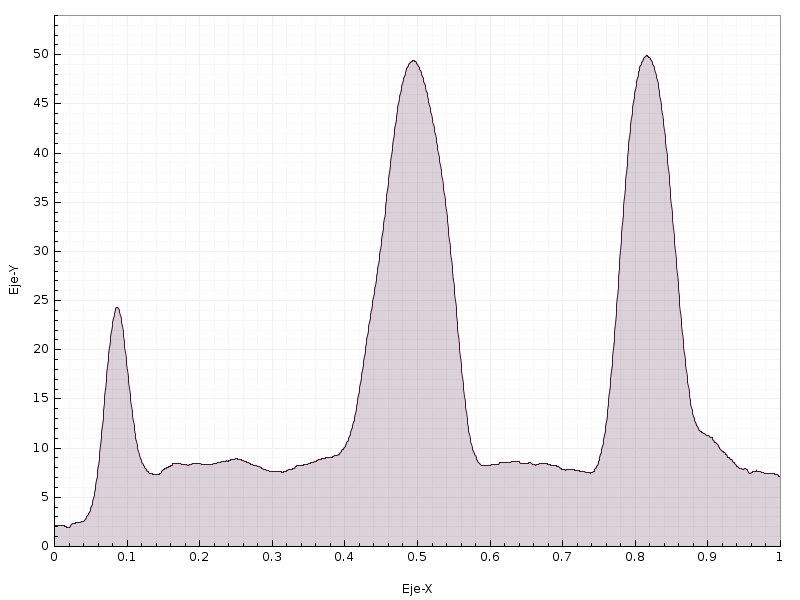
\includegraphics[width=230px]{imagenes-jtlc/experimento/search-peaks/4/plot-x}
	  \centering
	  \vspace{-0.4cm}
	  \caption{Plot de media sobre im\'agen con efectos en eje X.}
	  \label{fig:sp-4-plot-x-no-blur---repetido}
	  \vspace{-0.15cm}
	\end{figure}
	\begin{figure}[H]
	  \vspace{-0.2cm}
	  \centering
	  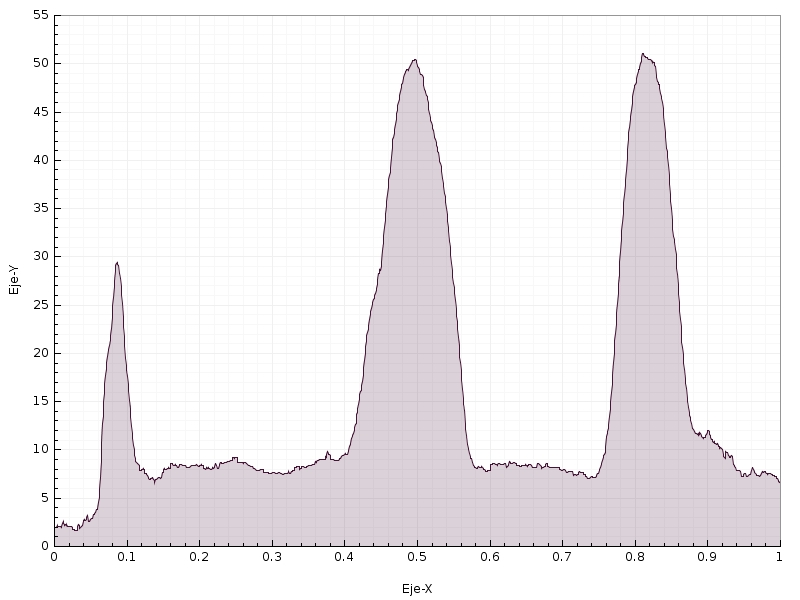
\includegraphics[width=230px]{imagenes-jtlc/experimento/search-peaks/4/plot-x-no-blur}
	  \centering
	  \vspace{-0.4cm}
	  \caption{Plot de media sobre im\'agen con efectos (sin blur) en eje X.}
	  \label{fig:sp-4-plot-x-no-blur}
	  \vspace{-0.15cm}
	\end{figure}
	Picos encontrados: \\
	(0.424, 0.5786667)\\ 
	(0.7493333, 0.8791111) \\ \\
	Picos encontrados (sin blur): \\
	(0.408, 0.576)\\
	(0.74755555, 0.88622224)\\
	
	\newpage
	\item \textit{B\'usqueda de picos (muestra 5)}
	\begin{figure}[H]
	\centering
	\fbox{
\includegraphics[width=40px]{imagenes-jtlc/experimento/search-peaks/5/1-blur}}   
	\hspace{30px}
	\fbox{
\includegraphics[width=40px]{imagenes-jtlc/experimento/search-peaks/5/2-gray}}
	\hspace{30px}
	\fbox{
\includegraphics[width=40px]{imagenes-jtlc/experimento/search-peaks/5/3-invert}}
	\caption{Aplicaci\'on de filtros sobre im\'agen de la muestra}
	\centering
	\end{figure}
	\begin{figure}[H]
	  \vspace{-0.2cm}
	  \centering
	  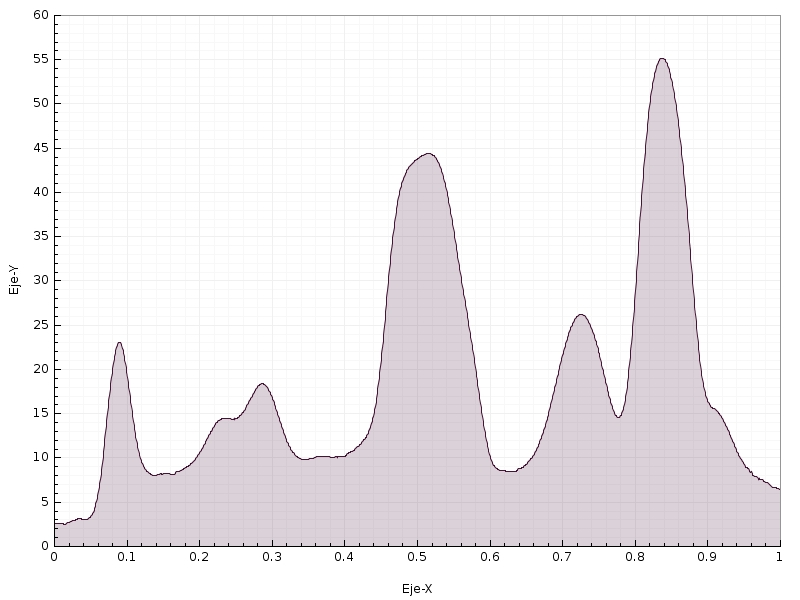
\includegraphics[width=230px]{imagenes-jtlc/experimento/search-peaks/5/plot-x}
	  \centering
	  \vspace{-0.4cm}
	  \caption{Plot de media sobre im\'agen con efectos en eje X.}
	  \label{fig:sp-5-plot-x-no-blur--repetido}
	  \vspace{-0.15cm}
	\end{figure}
	\begin{figure}[H]
	  \vspace{-0.2cm}
	  \centering
	  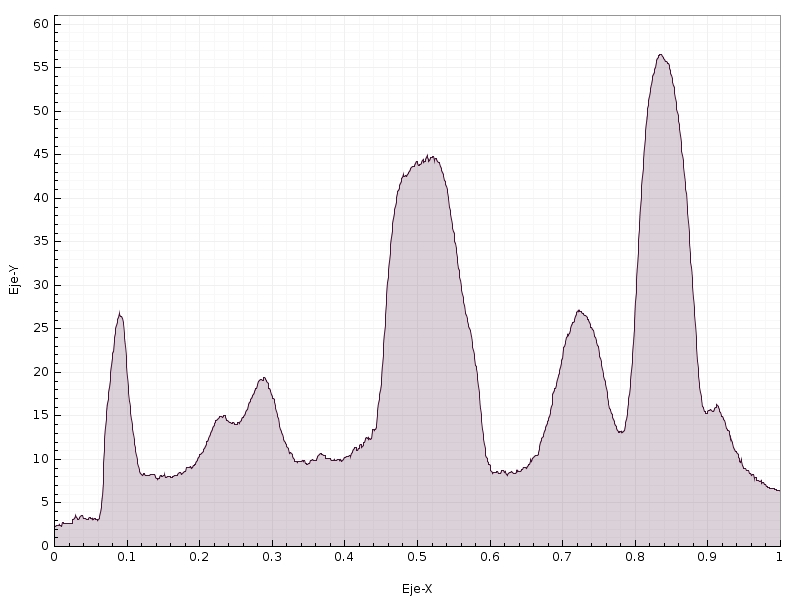
\includegraphics[width=230px]{imagenes-jtlc/experimento/search-peaks/5/plot-x-no-blur}
	  \centering
	  \vspace{-0.4cm}
	  \caption{Plot de media sobre im\'agen con efectos (sin blur) en eje X.}
	  \label{fig:sp-5-plot-x-no-blur}
	  \vspace{-0.15cm}
	\end{figure}
	Picos encontrados: \\
	(0.4471111, 0.5982222)\\
	(0.7831111, 0.9342222)\\ \\
	Picos encontrados (sin blur):\\
	(0.7857778, 0.8968889)\\
	
	\newpage
	\item \textit{B\'usqueda de picos (muestra 6)}
	\begin{figure}[H]
	\centering
	\fbox{
\includegraphics[width=40px]{imagenes-jtlc/experimento/search-peaks/6/1-blur}}   
	\hspace{30px}
	\fbox{
\includegraphics[width=40px]{imagenes-jtlc/experimento/search-peaks/6/2-gray}}
	\hspace{30px}
	\fbox{
\includegraphics[width=40px]{imagenes-jtlc/experimento/search-peaks/6/3-invert}}
	\caption{Aplicaci\'on de filtros sobre im\'agen de la muestra}
	\centering
	\end{figure}
	\begin{figure}[H]
	  \vspace{-0.2cm}
	  \centering
	  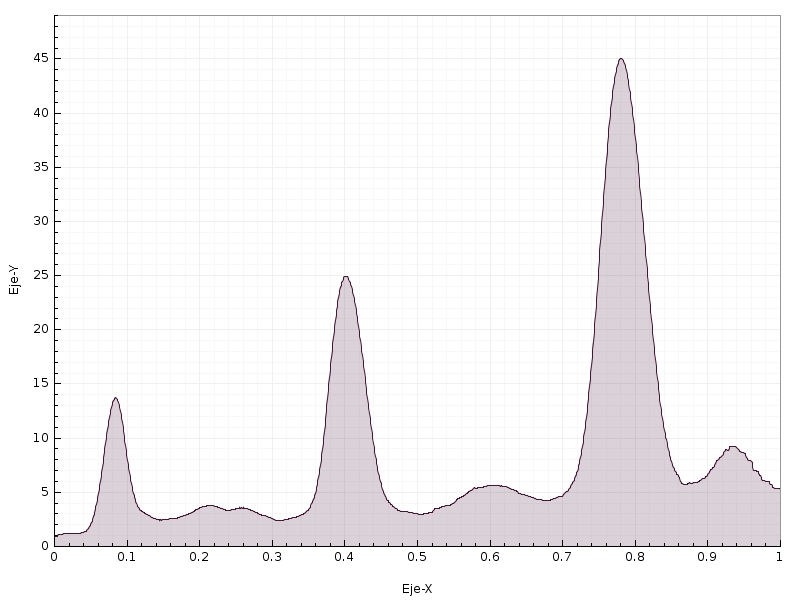
\includegraphics[width=230px]{imagenes-jtlc/experimento/search-peaks/6/plot-x}
	  \centering
	  \vspace{-0.4cm}
	  \caption{Plot de media sobre im\'agen con efectos en eje X.}
	  \label{fig:sp-6-plot-x-no-blur--repetido}
	  \vspace{-0.15cm}
	\end{figure}
	\begin{figure}[H]
	  \vspace{-0.2cm}
	  \centering
	  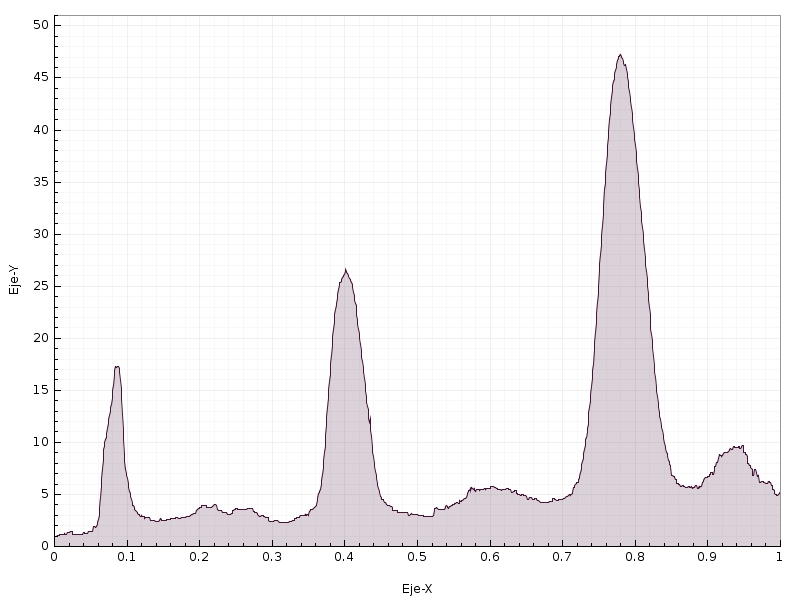
\includegraphics[width=230px]{imagenes-jtlc/experimento/search-peaks/6/plot-x-no-blur}
	  \centering
	  \vspace{-0.4cm}
	  \caption{Plot de media sobre im\'agen con efectos (sin blur) en eje X.}
	  \label{fig:sp-6-plot-x-no-blur}
	  \vspace{-0.15cm}
	\end{figure}
	Picos encontrados: \\
	(0.7271111, 0.8622222)\\ \\
	Picos encontrados (sin blur): \\
	(0.72977775, 0.8613333) \\
	
\end{itemize}
